\documentclass[11pt]{article}

% ---------- Papel tamano carta y margenes ----------
\usepackage[letterpaper,
left=2cm, right=2cm,
top=2cm, bottom=2cm]{geometry}

\usepackage[utf8]{inputenc}
\usepackage[spanish]{babel}
\usepackage[T1]{fontenc}
\usepackage{tikz}
\usepackage{array}
\usepackage{lastpage}
\usepackage{fancyhdr}
\usepackage[absolute,overlay]{textpos}
\usepackage{graphicx}
\usepackage{transparent}
\usepackage{eso-pic}
\begin{document}


\begin{titlepage}
    \AddToShipoutPictureBG*{%
	\AtPageLowerLeft{%
		\hspace*{11.5cm}%
		\raisebox{1cm}{%
			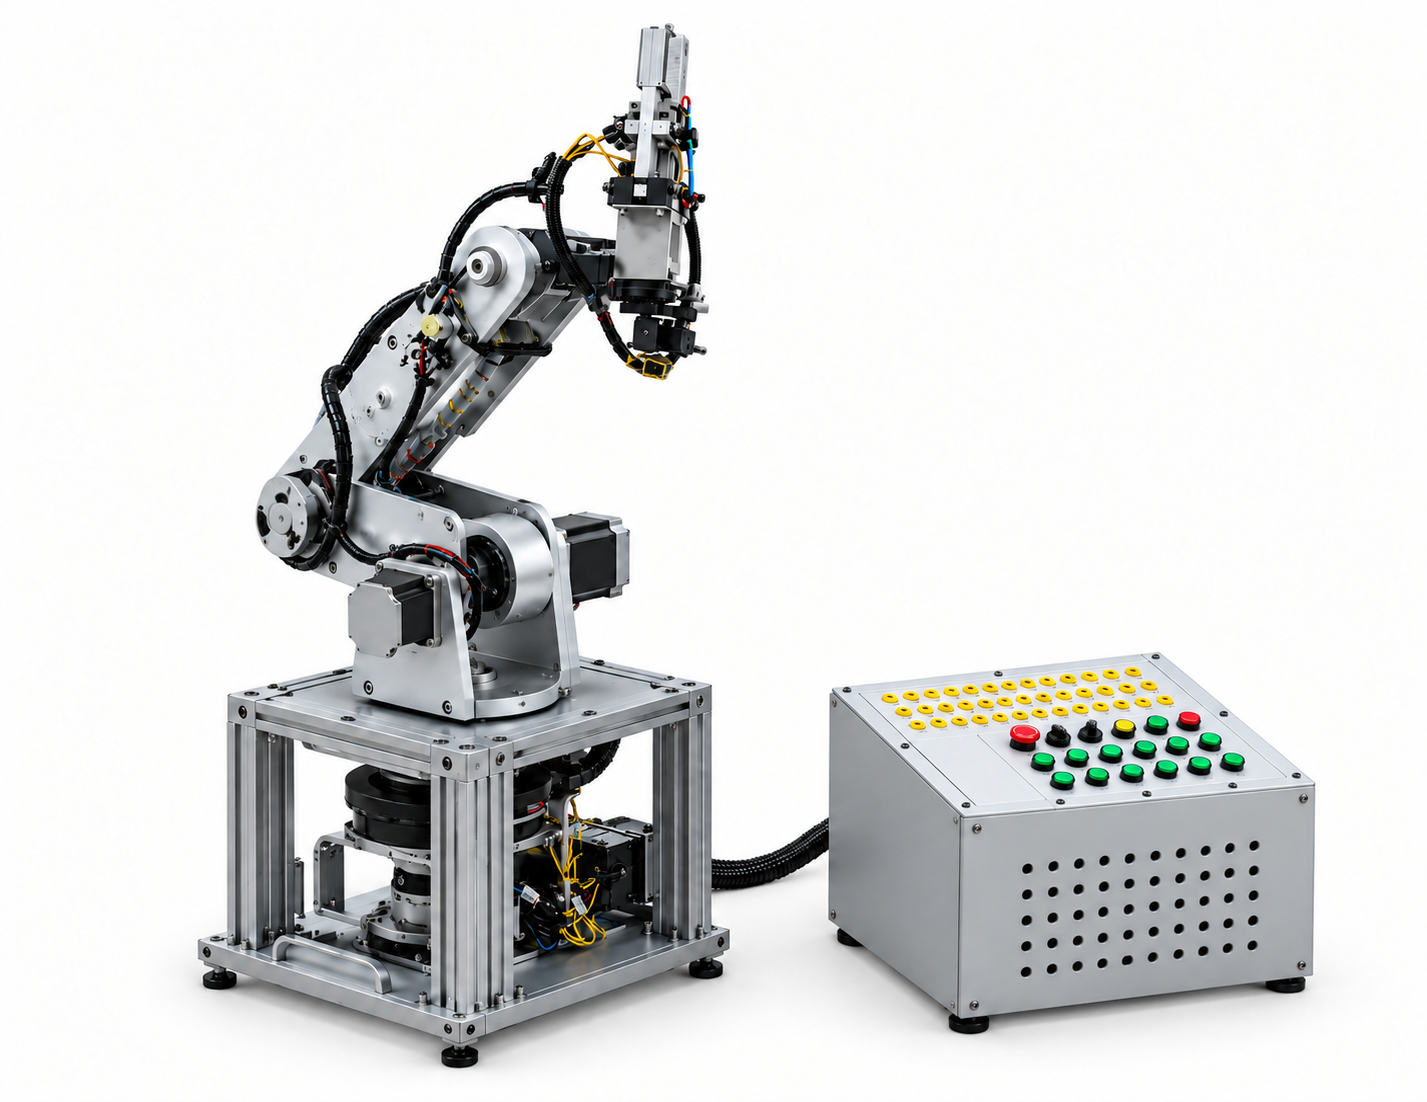
\includegraphics[width=10cm]{brazo.png}%
		}%
	}%
}
	\centering
	
	% Encabezado institucional
	{\fontsize{18}{24}\selectfont 
		UNIVERSIDAD MAYOR DE SAN ANDRÉS \\
		FACULTAD DE INGENIERÍA \\
		CARRERA DE INGENIERÍA ELECTRÓNICA \par}
	
	\vspace{0.5cm}
	
	% Logo 
	
\includegraphics[width=0.25\textwidth]{Umsa-logo.svg.png}
	
	% Título del informe
	\rule{\textwidth}{0.5pt} % Línea decorativa
	{\Huge\bfseries \\ INFORME DE LABORATORIO 1 \par}
	\rule{\textwidth}{0.5pt} % Línea decorativa
	{\Large\bfseries \\ETN-902, ETN-1000, ETN-1034\par}

	
	% Sección de integrantes
\begin{flushleft}
		{\Large\bfseries ESTUDIANTES: \par}
	\vspace{0.2cm}
	{\large
		\begin{tabular}{l}
			UNIV. CALLATA BAUTISTA DANIELA JHANIN\\
			UNIV. CARI ULURI CRISTHIAN DANIEL\\
			UNIV. GUTIERREZ PONCE CHRISTIAN YAMIL\\
			UNIV. MORALES CORICO NATALIA KATERINA\\
			UNIV. NINA FERNANDEZ DIEGO JOSUE\\
			UNIV. VILLCA YARARI GIOVANNI ALEXANDER
		\end{tabular} \par}
	\vspace{0.4cm}

	
	% Sección de docente
	{\Large\bfseries DOCENTE: \par}
	\vspace{0.2cm}
	{\large
		\begin{tabular}{l}
			ING. JORGE ANTONIO NAVA AMADOR
		\end{tabular} \par}

	\vspace{0.4cm}
	
	% Sección de auxiliares
	{\Large\bfseries AUXILIARES: \par}
	\vspace{0.2cm}
	{\large
		\begin{tabular}{l}
			UNIV. FABIAN MANUEL PLATA VARGAS\\
			UNIV. LIMBER AJNOTA CAHUAYA\\
			UNIV. FRANZ CHOQUE
		\end{tabular} \par}
	\end{flushleft}

	% Pie de página
	{\large 
		La Paz - Bolivia }
\end{titlepage}
\newpage

\tableofcontents
\newpage

\section{Introducci\'on}
	Texto de introducci\'on del informe de laboratorio o pr\'actica de
	Ingenier\'ia Electr\'onica. Reemplazar por el contenido real.
	
	\section{Objetivos}
	\begin{itemize}
		\item Objetivo general.
		\item Objetivos espec\'ificos.
	\end{itemize}
	
	\section{Marco Te\'orico}
	Contenido del marco te\'orico.
	
	\section{Desarrollo / Procedimiento}
	Descripci\'on del procedimiento experimental o desarrollo del tema.
	
	\section{Resultados}
	Presentaci\'on de resultados, tablas, gr\'aficos, mediciones.
	
	\section{Conclusiones}
	Conclusiones del trabajo realizado.
	
	\newpage
	\section{Anexos}
	Diagramas, c\'odigo fuente, hojas de datos, etc.
	
	
	
	El presente informe corresponde a la primera actividad de laboratorio del semestre II/2026, enfocada en la auditoría física y documental del Brazo Robótico de 6 Grados de Libertad (modelo de entrenamiento XK-LS5B). El trabajo se enmarca en la metodología Kaizen, realizando ingeniería inversa sobre la instrumentación, el mapeo de variables del sistema y la comparación entre la documentación heredada del semestre anterior y el equipo físico real.

\section{Objetivos}

\subsection*{Mención Control Automático (ETN-902)(ETN-1034)}

\begin{itemize}
	\item \textbf{Abstracción y Fenomenología:} Desarrollar la capacidad de identificar y clasificar las variables fundamentales en sistemas mecánicos, hidráulicos y de procesos del laboratorio.
	\item \textbf{Ingeniería Inversa:} Localizar y caracterizar físicamente los componentes de hardware (sensores ópticos, inductivos, de presión, actuadores paso a paso, variadores e interfaces PLC) sin depender de manuales de fábrica inexistentes.
	\item \textbf{Análisis de Causalidad:} Diagramar el proceso mediante bloques funcionales, estableciendo la relación causa-efecto entre las variables manipuladas (MV), variables controladas (PV) y variables de perturbación (DV), determinando las limitantes de operación en lazo abierto original.
\end{itemize}

\subsection*{Mención Bases de Datos (ETN-1000)}

\begin{itemize}
	\item \textbf{Análisis de Arquitectura:} Analizar los fundamentos técnicos de la comunicación y transferencia de datos entre elementos de procesamiento de campo (PLCs, RTUs) y un entorno cliente-servidor bajo el modelo estructural de 3 capas.
	\item \textbf{Análisis de Causalidad:} Investigar y contrastar las capacidades operativas y de latencia del hardware local del laboratorio frente a la viabilidad de despliegue de un backend en una PC industrial.
\end{itemize}

\section{Fuentes de Información Consultadas}

A diferencia de otras plantas del laboratorio, para el Brazo Robótico de 6 Grados de Libertad no se contó con un repositorio GitHub del docente con material vigente para el presente semestre. La única fuente disponible fue el informe de laboratorio del semestre anterior (Laboratorio 1, ETN-902/ETN-1034), el cual documenta la identificación previa de sensores, actuadores y controlador, y sirve como activo histórico de comparación. El docente indicó que, al no existir material actualizado para esta gestión, corresponde al presente grupo generar la documentación vigente de la planta a partir de la auditoría física realizada.

\section{Marco teórico}

\subsection{Sistema}

Un sistema es un conjunto de elementos interrelacionados que interactúan entre sí para cumplir un objetivo común.

Desde el punto de vista de control automático, un sistema puede representarse matemáticamente como una relación entre:

\begin{itemize}
	\item Entrada
	\item Proceso
	\item Salida
\end{itemize}

En el caso del brazo robótico de 6 GDL:

\begin{itemize}
	\item \textbf{Entrada:} Ángulo deseado.
	\item \textbf{Proceso:} Dinámica mecánica y eléctrica del brazo.
	\item \textbf{Salida:} Posición angular del brazo.
\end{itemize}

Un sistema puede clasificarse como:

\begin{itemize}
	\item Sistema dinámico (porque evoluciona en el tiempo).
	\item Sistema multivariable (porque tiene 6 entradas y 6 salidas).
	\item Sistema no lineal (debido a fricción, acoplamiento dinámico y gravedad).
\end{itemize}

\subsection{Planta}

La planta es la parte física del sistema que se desea controlar. En un brazo robótico de 6 GDL, la planta está compuesta por:

\begin{itemize}
	\item Estructura mecánica (eslabones y articulaciones)
	\item Motores eléctricos
	\item Reductores
	\item Transmisiones
	\item Carga manipulada
\end{itemize}

Modelar una planta en control implica crear una representación matemática (ecuaciones diferenciales, funciones de transferencia o espacio de estados) que describa la relación dinámica entre las entradas (acciones de control/perturbaciones) y salidas de un sistema físico. Se logra mediante modelado físico-matemático, identificación experimental o linealización, y comúnmente usando herramientas como MATLAB.

\subsubsection{Métodos de Modelado}

\begin{itemize}
	\item \textbf{Modelado Físico/Primeros Principios:} Se derivan ecuaciones diferenciales basadas en leyes físicas (ej. leyes de Newton para mecánica, Kirchhoff para circuitos).
	\item \textbf{Identificación de Sistemas:} Se aplican entradas conocidas (escalón, señal) al sistema real y se analiza la respuesta de salida para ajustar un modelo matemático.
	\item \textbf{Linealización:} Si el sistema es no lineal, se aproxima a un modelo lineal alrededor de un punto de operación específico para simplificar el control.
\end{itemize}

\subsubsection{Representaciones Comunes}

\begin{itemize}
	\item \textbf{Función de Transferencia (TF):} Modela sistemas lineales invariantes en el tiempo (LTI) en el dominio de Laplace, relacionando salida/entrada (ej. tf(num, den) en MATLAB).
	\item \textbf{Espacio de Estados (SS):} Utiliza matrices (A, B, C, D) para representar sistemas multivariables (MIMO) o más complejos, definiendo cómo evolucionan los estados internos.
\end{itemize}

\subsubsection{Pasos Típicos en la Práctica}

\begin{enumerate}
	\item Definir Entradas/Salidas: Identificar variables manipuladas, salidas a controlar y perturbaciones.
	\item Obtener Ecuaciones: Derivar el modelo matemático o realizar pruebas experimentales.
	\item Implementar en Software: Utilizar entornos como MATLAB/Simulink para definir la función de transferencia (tf) o espacio de estados (ss).
	\item Validar: Comparar la respuesta del modelo ante un escalón con el sistema real.
\end{enumerate}

\subsection{Proceso}

El proceso es el fenómeno físico que ocurre dentro de la planta. En el brazo robótico el proceso consiste en:

\begin{itemize}
	\item Movimiento angular de cada articulación.
	\item Posicionamiento espacial del efector final.
\end{itemize}

El proceso describe el comportamiento dinámico real del sistema.

\subsection{Variable}

Una variable es una magnitud física que puede cambiar en el tiempo y que describe el estado del sistema. En el brazo robótico tenemos:

\begin{itemize}
	\item Posición angular ($\theta$)
	\item Torque ($\tau$)
	\item Corriente del motor ($I$)
\end{itemize}

Las variables pueden ser:

\begin{itemize}
	\item Internas (estados del sistema)
	\item Externas (entrada o salida)
\end{itemize}

\subsection{Variable Manipulada (MV)}

Es la variable que el controlador modifica para influir en el sistema. En el brazo robótico:

\begin{itemize}
	\item Voltaje aplicado al motor
	\item Señal PWM
	\item Corriente de excitación
\end{itemize}

Se representa como: $u(t)$. Es la herramienta que usa el controlador para reducir el error.

\subsection{Variable Controlada (PV)}

Es la variable que se desea mantener en un valor específico. En el brazo robótico:

\begin{itemize}
	\item Posición angular deseada de cada articulación.
	\item Posición cartesiana del efector final.
\end{itemize}

Se representa como: $y(t)$. Es la salida del sistema que se mide mediante sensores.

\subsection{Referencia (Setpoint)}

Es el valor deseado de la variable controlada: $r(t)$.

\subsection{Error}

Es la diferencia entre la referencia y la salida real:

\begin{equation}
	e(t) = r(t) - y(t)
\end{equation}

El controlador actúa en función del error. Si $e(t) = 0 \Rightarrow$ Sistema en equilibrio; si $e(t) \neq 0 \Rightarrow$ El controlador actúa.

\subsection{Perturbación (DV)}

Es una señal externa que afecta el comportamiento del sistema sin pasar por el controlador. Ejemplos en el brazo robótico:

\begin{itemize}
	\item Peso adicional en el efector final.
	\item Vibraciones externas.
	\item Variaciones de voltaje en la fuente.
\end{itemize}

Se representa como: $d(t)$. Un buen sistema de control debe minimizar el efecto de las perturbaciones.

\subsection{Retroalimentación (Feedback)}

Es el proceso mediante el cual la salida del sistema se mide y se compara con la referencia. En el brazo robótico:

\begin{enumerate}
	\item El encoder mide la posición real.
	\item Se envía al controlador.
	\item Se calcula el error.
	\item Se corrige la señal de control.
\end{enumerate}

La retroalimentación permite: mayor precisión, estabilidad, corrección automática de errores y rechazo de perturbaciones.

\subsection{Sistema de Lazo Abierto}

No existe retroalimentación.

No corrige errores.

\subsection{Sistema de Lazo Cerrado}

Existe retroalimentación.

Permite corregir errores continuamente.

\section{Descripción del Sistema}

El brazo robótico de 6 GDL está compuesto por seis articulaciones independientes: base rotacional, hombro, codo y tres articulaciones en la muñeca. Cada articulación posee un actuador y un sensor de posición.

\subsection{Brazo robótico de seis grados de libertad – modelo de entrenamiento XK-LS5B}

El XK-LS5B es un brazo robótico de entrenamiento de seis grados de libertad (6 GDL), diseñado para el estudio y la práctica de conceptos fundamentales de robótica. Sus seis grados de libertad permiten controlar tanto la posición como la orientación del efector final dentro del espacio de trabajo. Los movimientos principales pueden asociarse con la rotación de la base, el movimiento de los diferentes eslabones y la orientación de la muñeca. De esta manera, el robot puede desplazar y orientar una herramienta o pinza en diferentes direcciones.

Una característica importante de un robot de 6 GDL es que permite describir la posición y orientación del efector final mediante seis variables independientes:



donde $q_1, \ldots, q_6$ representan las variables articulares correspondientes a cada grado de libertad.

Los robots de estas características son utilizados como plataformas educativas para estudiar cinemática directa, cinemática inversa, transformación de coordenadas, control de motores y generación de trayectorias.

\subsubsection{Base del Robot (Eje 1)}

Constituye la estructura de soporte y aloja la primera articulación. El actuador es un motor paso a paso que, acoplado a un sistema de transmisión por poleas, genera el par motor necesario para el movimiento de rotación de la torre (brazo completo) en el plano horizontal. Se incorpora un codificador rotativo como sensor de posición para el control en lazo cerrado, permitiendo registrar el ángulo de giro y realimentar al controlador.

\subsubsection{Cadena Cinemática (Brazo)}

Compuesta por los eslabones que definen los grados de libertad restantes:

\begin{itemize}
	\item \textbf{Articulación del Hombro (Eje 2):} El brazo grande actúa como eslabón. Un motor paso a paso, ubicado en su eje inferior (articulación), funciona como actuador directo para controlar la rotación del brazo grande en el plano vertical.
	
	\item \textbf{Articulación del Codo (Eje 3):} El brazo pequeño es el eslabón siguiente. Su actuador (otro motor paso a paso) se encuentra en el eje del hombro y transmite el par motor al codo mediante una transmisión por correa síncrona, controlando así la rotación del brazo pequeño.
	
	\item \textbf{Efector Final (Muñeca y Pinza):}
	\begin{itemize}
		\item \textbf{Articulación de la Muñeca (Eje 4):} Un motor paso a paso en el lado del brazo pequeño, acoplado a una transmisión síncrona, comanda la rotación completa (giro) de la pata (antebrazo y muñeca).
		\item \textbf{Articulación de la Pinza (Eje 5):} Un motor paso a paso en el centro de la pata actúa como actuador para el control de apertura/cierre de los dedos (actuación de la pinza).
		\item \textbf{Articulación de Giro de Muñeca (Eje 6):} Un motor paso a paso en el extremo de la pata, acoplado a un reductor de velocidad, genera el par necesario para el control de la rotación fina de la muñeca (último grado de libertad).
	\end{itemize}
\end{itemize}

\section{Identificación de Componentes}

\subsection{Sensores}

\subsubsection{Sensor de Final de Carrera Mecánico – Modelo M102-011}

Se encontraron 2 en la pinza. Dispositivo electromecánico o electrónico que detecta cuando un mecanismo llega a una posición límite predeterminada.



\begin{itemize}
	\item \textbf{Principio:} Interruptor SPDT con un accionador mecánico.
	\item \textbf{Características:} Contactos: Común (COM), Normalmente Abierto (NO), Normalmente Cerrado (NC).
	\item \textbf{Corriente:} 5A a 250 VAC / 3A a 125 VAC.
	\item \textbf{Polos:} SPDT. Pines: 3 (NO, COM, NC). Largo de palanca: 19 mm. Tiempo de conmutación: 1.9 ms.
	\item \textbf{Función:} Detectar los límites de apertura y cierre de la garra.
\end{itemize}

Se utiliza para: detectar fin de recorrido, evitar sobrecarreras, referencia de posición inicial (home). Funciona generalmente por contacto físico (micro-switch), aunque también puede ser óptico o magnético.

\subsubsection{Sensor Magnético (Efecto Hall) – Modelo NJK-5002C}

Se encontraron 5 unidades. Sensor que detecta la presencia o variación de un campo magnético.

\begin{itemize}
	\item \textbf{Principio:} Detecta la presencia de un campo magnético (de los imanes circulares en las articulaciones). Cuando se acerca un imán, conmuta su salida.
	\item \textbf{Características:} NPN, Normalmente Abierto (NO), 3 hilos (Marrón: VCC 6–36V, Negro: Salida, Azul: GND). Distancia de detección: 10 mm.
	\item \textbf{Voltaje de operación:} 6–36 V DC. Consumo: 300 mA. Frecuencia de respuesta: 100 Hz.
	\item \textbf{Función:} Actúan como fines de carrera, indicando al PIC que una articulación ha llegado al límite de su recorrido. El informe previo verificó su conmutación en 1.9 ms.
\end{itemize}

Tipos comunes: Efecto Hall, Reed switch. Aplicaciones: detección de posición, medición de velocidad, detección de proximidad sin contacto. Ventaja: no hay desgaste mecánico.

\subsubsection{Sensor resistivo lineal y angular}

Dispositivo cuya resistencia varía según la posición.

\begin{itemize}
	\item \textbf{Lineal:} Potenciómetro lineal (mide desplazamiento en línea recta).
	\item \textbf{Angular:} Potenciómetro rotatorio (mide ángulo de giro).
\end{itemize}

Funcionamiento: al variar la posición del cursor cambia el voltaje de salida (divisor de tensión). Son simples y económicos, pero sufren desgaste mecánico.

\subsubsection{Encoder incremental – Modelo MBL3806-AB-600-24C}

Sensor que convierte movimiento mecánico en pulsos digitales.

\begin{itemize}
	\item \textbf{Tipo:} Incremental Óptico. PPR: 600. Voltaje de operación: 5–24 V DC.
	\item \textbf{Salida:} NPN colector abierto, dos fases (AB). Frecuencia de respuesta: 20 KHz.
	\item \textbf{Velocidad máxima mecánica:} 5000 RPM.
	\item \textbf{Conexiones:} Rojo: VCC (5–24V), Negro: GND (0V), Verde: Fase A, Blanco: Fase B.
\end{itemize}

Características: Genera trenes de pulsos (canales A y B desfasados 90°). Permite medir: velocidad, dirección, posición relativa. No da posición absoluta, necesita referencia inicial (home). Muy usado en motores y sistemas CNC.

\subsection{Actuadores}

\subsubsection{Driver (2M542-N)}

Recibe las señales MV de baja potencia (PUL, DIR). Su circuito interno (optoacoplado) las aísla y las utiliza para controlar transistores MOSFET que conmutan la corriente de alta potencia (24V, hasta 4.2A) desde la fuente conmutada hacia las bobinas del motor.

Los controladores 4OKF y O4IFJJ son dispositivos utilizados para controlar y manejar motores de pasos bipolares en diferentes aplicaciones; entre sus principales funciones dentro del brazo permiten controlar la corriente suministrada al motor paso a paso. Esto es importante para garantizar un rendimiento óptimo del motor y evitar sobrecalentamiento y daños.

\textbf{Configuración de subdivisión de micropasos:} El número de subdivisiones de micropasos del controlador se establece mediante cuatro interruptores DIP SW5-SW8, y hay 15 niveles de subdivisiones de micropasos en total. Cuando el usuario configura la subdivisión de micropasos, la unidad debe detenerse primero.

La corriente de salida del controlador se establece mediante tres interruptores DIP SW1-SW3 y hay 8 niveles de corriente de salida.

\subsubsection{Motor paso a paso}

Motor eléctrico que gira en incrementos angulares discretos (pasos).

\begin{itemize}
	\item \textbf{Características:} Movimiento preciso sin necesidad de sensor (en lazo abierto). Controlado por secuencia de pulsos.
	\item \textbf{Ideal para:} Impresoras 3D, CNC, Brazos robóticos.
	\item \textbf{Tipos:} Unipolar, Bipolar.
\end{itemize}

\subsubsection{NEMA 17}

No es el motor en sí, sino el estándar de tamaño según la norma National Electrical Manufacturers Association.

\begin{itemize}
	\item 1.7 pulgadas (43 mm) de lado frontal. Común en impresoras 3D. Torque medio.
	\item \textbf{Modelo:} 42J1848-604 D13.6 (6 hilos).
	\item \textbf{Especificaciones:} Ángulo de paso 1.8° (200 pasos/rev), Corriente 1.2A, Par 3.2 kg-cm, Resistencia de bobina variable según conexión (serie o centro). Se midió, por ejemplo, 59.1$\Omega$ entre rojo-verde.
	\item \textbf{Aplicación:} Giro de muñeca (Joint 5) y apertura/cierre de pinza (Joint 6).
\end{itemize}

\subsubsection{NEMA 23}

También estándar NEMA, más grande que el 17.

\begin{itemize}
	\item 2.3 pulgadas (57 mm) de lado frontal. Mayor torque. Usado en CNC y sistemas industriales pequeños.
	\item \textbf{Modelo:} 57J1854-828 (bobina doble, 8 hilos).
	\item \textbf{Especificaciones:} Ángulo de paso 1.8° (200 pasos/rev), Corriente por fase 2.8A, Par de retención 0.9–1.9 Nm, Resistencia de bobina 2.2 $\Omega$ por fase.
	\item \textbf{Aplicación:} Movimiento de las articulaciones principales (base, brazo, antebrazo).
\end{itemize}

\subsection{Controlador}

\subsubsection{Microcontrolador PIC 16F1946}

Es el cerebro del sistema. Se encarga de leer los pulsadores del tablero y los sensores, ejecutar la lógica de control programada y generar las señales digitales de baja potencia (PUL, DIR, EN) para los drivers.

Características: Memoria Flash de 14KB, 54 pines de E/S, oscilador interno, conversor ADC de 10 bits.

Microcontrolador de 8 bits fabricado por Microchip Technology.



Aplicaciones: Control de motores, lectura de sensores, automatización embebida.

\subsection{Tabla de Referencia N°1}

Reconocer físicamente los elementos que constituyen un lazo de control: sensores, actuadores y controladores.



\section{Clasificación de Variables}

\subsection{Referencia (r)}

Es la señal que define el valor deseado para la Variable Controlada (PV). En un sistema de control, es el objetivo que se quiere alcanzar. En el brazo robótico de 6 GDL, el operador establece la referencia a través del tablero de control. Esta referencia puede ser:

\begin{itemize}
	\item Posición cartesiana deseada del efector final: $(x_d, y_d, z_d)$
	\item Orientación deseada: $(\phi_d, \theta_d, \psi_d)$
	\item Ángulos articulares deseados: $\theta_{1d}, \theta_{2d}, \theta_{3d}, \theta_{4d}, \theta_{5d}, \theta_{6d}$
\end{itemize}

Para el análisis y control de este sistema, se define como señal de entrada $r(t)$ al vector de posiciones angulares deseadas por cada grado de libertad. Esta es la entrada de referencia al sistema de control.

\subsection{Variable Controlada (PV – Process Variable): $y(t)$}

Es la magnitud física que se mide y se desea controlar, en nuestro caso posición angular en el brazo. En el brazo robótico: posición angular real de cada articulación $\theta_1, \theta_2, \theta_3, \theta_4, \theta_5, \theta_6$. En nuestro sistema multivariable hay 6 variables controladas simultáneamente.

\subsection{Variable Manipulada (MV): $u(t)$}

Es la variable que el controlador puede modificar para corregir el sistema. En el brazo de 6 grados de libertad, el PIC interpreta la referencia y, basado en su lógica interna (y considerando si se ha activado algún sensor de límite), genera dos señales digitales clave que conforman la Variable Manipulada (MV):

\begin{itemize}
	\item \textbf{PUL (Pulso):} Un tren de ondas cuadradas (PWM). La cantidad de pulsos determina la posición angular objetivo (cuántos pasos debe girar el motor). La frecuencia de los pulsos determina la velocidad de giro.
	\item \textbf{DIR (Dirección):} Un nivel lógico constante (0V o 5V) que define el sentido de giro del motor (horario o antihorario).
	\item En algunos casos, también se usa una señal \textbf{ENA (Enable)} para habilitar o deshabilitar el driver.
\end{itemize}

Matemáticamente: $u_1(t), u_2(t), u_3(t), u_4(t), u_5(t), u_6(t)$. Cada articulación tiene su propia variable manipulada, por lo que la interpretaremos como un vector al igual que las entradas.

\subsection{Variable de Perturbación (DV – Disturbance Variable): $d(t)$}

Son variables externas que afectan el sistema y no son controladas directamente. En el brazo 6 GDL pueden ser debido a:

\begin{itemize}
	\item Peso del objeto manipulado
	\item Cambios en la carga
	\item Vibraciones externas
	\item Variación en la tensión de alimentación
\end{itemize}

Si el brazo levanta una pieza más pesada, el torque requerido cambia; eso es una perturbación.

\subsection{Tabla de Referencia N°2}

Identificar y diferenciar las variables del sistema: Variable Manipulada (MV), Variable Controlada (PV) y Variables de Perturbación (DV).



\subsection{Tabla de Variables del Sistema}



\subsection{Clasificación de Sensores por Principio Físico}

\section{Tipo de Sistema}

El sistema en laboratorio opera en lazo abierto, ya que es un sistema dinámico tal y como se nos presenta, pero si se utilizan los sensores para medir la posición y corregir continuamente el error mediante retroalimentación podemos convertir el sistema en uno de lazo cerrado.

\subsection{Diagrama de Bloques General}

\subsection{Diagrama de Bloques – Lazo Abierto}

Diagrama de bloques general del brazo robótico de 6 GDL en su configuración actual (lazo abierto). Se observa que la retroalimentación de los sensores magnéticos y mecánicos no se utiliza para calcular el error de posición, sino únicamente como protección (fines de carrera) y referencia inicial (homing).

\subsubsection{Eje 1 – Base}

Rotación horizontal. Motor NEMA23 · Driver 2M542-N · Sensor Hall NJK-5002C + encoder rotativo (encoder no conectado al PIC actualmente). Sistema en lazo abierto; $b_1(t)$ es protección, no retroalimentación.

\subsubsection{Eje 2 – Hombro}

Rotación vertical del brazo grande. Motor NEMA23 con acoplamiento directo al eje. Sistema en lazo abierto. No existe verificación de la posición alcanzada; si el motor pierde pasos por sobreesfuerzo, el error no se detecta.

\subsubsection{Eje 3 – Codo}

El motor NEMA23 está ubicado físicamente en el eje del hombro, pero su par se transmite al codo mediante una correa síncrona. La transmisión por correa puede introducir juego mecánico o deslizamiento, generando errores no detectados en lazo abierto.

\subsubsection{Eje 4 – Muñeca}

Actuador: motor NEMA 17 (menor torque que los NEMA 23). Efecto: rotación completa de la pata (antebrazo y muñeca). El menor torque del NEMA 17 lo hace más susceptible a pérdida de pasos por carga externa.

\subsubsection{Eje 5 – Pinza}

Actuador: motor NEMA 17 con driver 2MA320. Protección: dos finales de carrera mecánicos M102-011 detectan los límites de apertura y cierre. Los sensores solo detienen el movimiento al llegar al límite, no posicionan la pinza en puntos intermedios.

\subsubsection{Eje 6 – Giro de Muñeca / Pinza}

Único eje con dos sensores de fin de carrera mecánico M102-011 (SPDT): uno detecta el límite de cierre ($b_{6a}$) y el otro el de apertura ($b_{6b}$). Motor NEMA17 con driver 2MA320. En lazo abierto, el reductor puede introducir histéresis o backlash no compensado.

\subsection{Diagrama de Bloques – Lazo Cerrado}

El sistema actualmente opera en lazo abierto, pero cuenta con los componentes necesarios (encoders incrementales) para operar en lazo cerrado. Si se conectaran estos sensores al PIC, se obtendría el siguiente esquema:

\subsubsection{Eje 1 – Base (lazo cerrado)}

El encoder incremental (1000 pulsos/rev) mide $\theta_1$ real y lo retroalimenta al PIC, que calcula $e_1(t) = \theta_{1d} - \hat{\theta}_1$ y corrige la señal PUL/DIR. Transmisión por poleas.

\subsubsection{Eje 2 – Hombro (lazo cerrado)}

Motor NEMA 23 con acoplamiento directo al eje. El encoder mide $\theta_2$ real y cierra el lazo de posición angular: $e_2(t) = \theta_{2d} - \theta_{2,real}$.

\subsubsection{Eje 3 – Codo (lazo cerrado)}

Encoder instalado en el codo mide la posición real: $e_3(t) = \theta_{3d} - \theta_{3,real}$. El sistema compensa errores por holgura de la correa o fricción. El lazo cerrado es especialmente relevante en este eje debido a la transmisión indirecta (correa), más propensa a errores que el acoplamiento directo.

\subsubsection{Eje 4 – Muñeca (lazo cerrado)}

$e_4(t) = \theta_{4d} - \theta_{4,real}$. Retroalimentación: encoder en el eje de muñeca. Corrección continua ante perturbaciones como el peso de un objeto manipulado.

\subsubsection{Eje 5 – Pinza (lazo cerrado)}

$e_5(t) = \theta_{5d} - \theta_{5,real}$. Se podría usar un potenciómetro (ya existente) o encoder para medir la apertura real, permitiendo sujetar objetos con la fuerza justa sin aplastarlos, o posicionar la pinza en aperturas intermedias.

\subsubsection{Eje 6 – Giro de Muñeca (lazo cerrado)}

$e_6(t) = \theta_{6d} - \theta_{6,real}$. Retroalimentación: potenciómetro (señal analógica 0-5V) o encoder. El PIC lee el valor del potenciómetro a través de su ADC de 10 bits y corrige la posición.

\subsection{Causalidad}

Los diagramas de causalidad muestran la relación causa-efecto entre las señales que intervienen en el sistema, identificando:

\begin{itemize}
	\item \textbf{Causa:} Señal de entrada o acción que origina un efecto.
	\item \textbf{Efecto:} Resultado o respuesta del sistema ante esa causa.
	\item \textbf{Retroalimentación:} Flujo de información desde la salida hacia la entrada (solo en lazo cerrado).
\end{itemize}

\subsubsection{Lazo Abierto}

En lazo abierto, el PIC envía pulsos sin verificar la posición real:

\paragraph{Eje 1 (Base) – Lazo Abierto}
\begin{itemize}
	\item \textbf{Causa (entrada):} El operador ingresa un ángulo deseado $\theta_{1d}$ mediante el tablero de control.
	\item \textbf{Proceso:} El PIC genera una cantidad específica de pulsos (PUL) y una señal de dirección (DIR).
	\item \textbf{Efecto (salida):} El motor NEMA 23 gira un número proporcional de pasos, moviendo la base mediante poleas.
	\item \textbf{Limitación:} El sensor Hall NJK-5002C solo actúa como final de carrera (protección), no como retroalimentación continua. El encoder rotativo existe pero no está conectado al PIC.
	\item \textbf{Causalidad:} La señal PUL (causa) produce un giro angular (efecto), sin verificación del resultado real.
\end{itemize}

\paragraph{Eje 2 (Hombro) – Lazo Abierto}
\begin{itemize}
	\item \textbf{Causa:} Señal de pulsos generada por el PIC según el ángulo deseado $\theta_{2d}$.
	\item \textbf{Proceso:} El motor NEMA 23 está acoplado directamente al eje del hombro (sin transmisión adicional).
	\item \textbf{Efecto:} El brazo grande rota en el plano vertical hasta la posición ordenada.
	\item \textbf{Limitación:} No existe verificación de la posición alcanzada. Si el motor pierde pasos por sobresfuerzo, el error no se detecta.
	\item \textbf{Causalidad:} PUL $\rightarrow \theta_2$ (unidireccional, sin retroalimentación).
\end{itemize}

\paragraph{Eje 3 (Codo) – Lazo Abierto}
\begin{itemize}
	\item \textbf{Causa:} Señal de control del PIC para el ángulo deseado $\theta_{3d}$.
	\item \textbf{Singularidad:} El motor está ubicado físicamente en el eje del hombro, pero su par se transmite al codo mediante una correa sincrónica.
	\item \textbf{Efecto:} El brazo pequeño (antebrazo) rota en el plano vertical.
	\item \textbf{Limitación:} La transmisión por correa puede introducir juego mecánico o deslizamiento, generando errores no detectados en lazo abierto.
	\item \textbf{Causalidad:} PUL $\rightarrow$ (transmisión por correa) $\rightarrow \theta_3$.
\end{itemize}

\paragraph{Eje 4 (Muñeca) – Lazo Abierto}
\begin{itemize}
	\item \textbf{Causa:} Señal de pulsos para el ángulo deseado $\theta_{4d}$.
	\item \textbf{Actuador:} Motor NEMA 17 (menor torque que los NEMA 23).
	\item \textbf{Efecto:} Rotación completa de la pata (antebrazo y muñeca).
	\item \textbf{Limitación:} El menor torque del NEMA 17 lo hace más susceptible a pérdida de pasos por carga externa.
	\item \textbf{Causalidad:} PUL $\rightarrow \theta_4$ (sin verificación).
\end{itemize}

\paragraph{Eje 5 (Pinza) – Lazo Abierto}
\begin{itemize}
	\item \textbf{Causa:} Señal de apertura o cierre deseado.
	\item \textbf{Actuador:} Motor NEMA 17 con driver 2MA320.
	\item \textbf{Efecto:} Movimiento de los dedos de la pinza.
	\item \textbf{Protección:} Dos finales de carrera mecánicos M102-011 detectan los límites de apertura y cierre.
	\item \textbf{Limitación:} Los sensores solo detienen el movimiento al llegar al límite, no posicionan la pinza en puntos intermedios.
	\item \textbf{Causalidad:} PUL $\rightarrow$ posición de pinza (abierto/cerrado o intermedio sin precisión).
\end{itemize}

\paragraph{Eje 6 (Giro de Muñeca) – Lazo Abierto}
\begin{itemize}
	\item \textbf{Causa:} Señal de pulsos para el ángulo deseado $\theta_{6d}$.
	\item \textbf{Actuador:} Motor NEMA 17 con reductor de velocidad (aumenta el torque pero reduce la velocidad).
	\item \textbf{Efecto:} Rotación fina de la muñeca (último grado de libertad).
	\item \textbf{Protección:} Sensor Hall NJK-5002C como final de carrera.
	\item \textbf{Limitación:} En lazo abierto, el reductor puede introducir histéresis o backlash no compensado.
	\item \textbf{Causalidad:} PUL $\rightarrow \theta_6$ (unidireccional).
\end{itemize}

\textbf{Leyenda:}
\begin{itemize}
	\item Causal directa
	\item Causal indirecta
	\item Perturbación $d(t)$
	\item Realimentación encoder
	\item Protección $b(t)$
	\item + efecto positivo
	\item – efecto negativo
\end{itemize}

\subsubsection{Lazo Cerrado}

\paragraph{Descripción General}
Se incorpora la medición del encoder para corregir errores:
\begin{itemize}
	\item $y(t)$ es medido por el encoder.
	\item El error $e(t) = r(t) - y(t)$ se actualiza continuamente.
	\item Lazo cerrado con control PID para rechazo de perturbaciones $d(t)$.
\end{itemize}

\paragraph{Eje 1 (Base) – Lazo Cerrado}
\begin{itemize}
	\item \textbf{Causa principal:} Ángulo deseado $\theta_{1d}$ (referencia).
	\item \textbf{Comparación:} Se calcula el error $e_1(t) = \theta_{1d} - \theta_{1real}$.
	\item \textbf{Acción correctiva:} El PIC genera pulsos proporcionales al error.
	\item \textbf{Retroalimentación:} El encoder incremental (1000 pulsos/rev) mide la posición real y la envía al PIC.
	\item \textbf{Efecto:} El sistema corrige automáticamente cualquier desviación por pérdida de pasos o perturbaciones.
\end{itemize}

\paragraph{Eje 2 (Hombro) – Lazo Cerrado}
\begin{itemize}
	\item \textbf{Causa inicial:} Ángulo deseado $\theta_{2d}$.
	\item \textbf{Error:} $e_2(t) = \theta_{2d} - \theta_{2real}$.
	\item \textbf{Retroalimentación:} El encoder mide la posición real del hombro.
	\item \textbf{Efecto corregido:} El PIC ajusta los pulsos hasta que el error sea cero.
\end{itemize}

\paragraph{Eje 3 (Codo) – Lazo Cerrado}
\begin{itemize}
	\item \textbf{Causa:} Referencia $\theta_{3d}$.
	\item \textbf{Error:} $e_3(t) = \theta_{3d} - \theta_{3real}$.
	\item \textbf{Retroalimentación:} Encoder instalado en el codo mide la posición real.
	\item \textbf{Efecto:} El sistema compensa errores por holgura de la correa o fricción.
	\item \textbf{Importancia:} El lazo cerrado es especialmente relevante en este eje debido a la transmisión indirecta (correa), que es más propensa a errores que el acoplamiento directo.
\end{itemize}

\paragraph{Eje 4 (Muñeca) – Lazo Cerrado}
\begin{itemize}
	\item \textbf{Causa:} $\theta_{4d}$.
	\item \textbf{Error:} $e_4(t) = \theta_{4d} - \theta_{4real}$.
	\item \textbf{Retroalimentación:} Encoder en el eje de muñeca.
	\item \textbf{Efecto:} Corrección continua ante perturbaciones como el peso de un objeto manipulado.
\end{itemize}

\paragraph{Eje 5 (Pinza) – Lazo Cerrado}
\begin{itemize}
	\item \textbf{Causa:} Apertura deseada (porcentaje o posición lineal).
	\item \textbf{Retroalimentación:} Se podría usar un potenciómetro (ya existente) o encoder para medir la apertura real.
	\item \textbf{Error:} $e_5(t) = \theta_{5d} - \theta_{5real}$.
	\item \textbf{Efecto:} Permite sujetar objetos con la fuerza justa sin aplastarlos, o posicionar la pinza en aperturas intermedias.
\end{itemize}

\paragraph{Eje 6 (Giro de Muñeca) – Lazo Cerrado}
\begin{itemize}
	\item \textbf{Causa:} $\theta_{6d}$.
	\item \textbf{Retroalimentación:} Potenciómetro (señal analógica 0–5V) o encoder.
	\item \textbf{Error:} $e_6(t) = \theta_{6d} - \theta_{6real}$.
	\item \textbf{Efecto:} El PIC lee el valor del potenciómetro a través de su ADC de 10 bits y corrige la posición.
\end{itemize}

\subsection{Descripción de Bloques del Sistema}

\begin{enumerate}
	\item \textbf{Entrada de Referencia ($r(t)$):} Es la acción del operador sobre el tablero de control. Puede ser:
	\begin{itemize}
		\item Un pulsador de mando manual (ej. M01 para giro derecha del Joint 1). La señal es de 24V DC, que pasa por optoacopladores para ser leída por el PIC a 5V.
		\item Un comando de un programa automático almacenado en el PIC (si el selector está en "Auto").
	\end{itemize}
	
	\item \textbf{Controlador (PIC 16F1946):} El PIC interpreta la referencia y, basado en su lógica interna (y considerando si se ha activado algún sensor de límite), genera dos señales digitales clave que conforman la Variable Manipulada (MV):
	\begin{itemize}
		\item \textbf{PUL (Pulso):} Un tren de ondas cuadradas (PWM). La cantidad de pulsos determina la posición angular objetivo (cuántos pasos debe girar el motor). La frecuencia de los pulsos determina la velocidad de giro.
		\item \textbf{DIR (Dirección):} Un nivel lógico constante (0V o 5V) que define el sentido de giro del motor (horario o antihorario).
	\end{itemize}
	En algunos casos, también se usa una señal ENA (Enable) para habilitar o deshabilitar el driver.
	
	\item \textbf{Actuador (Driver + Motor Paso a Paso):}
	\begin{itemize}
		\item \textbf{Driver:} Recibe las señales MV de baja potencia (PUL, DIR). Su circuito interno (optoacoplado) las aísla y las utiliza para controlar transistores MOSFET que conmutan la corriente de alta potencia (24V, hasta 4.2A) desde la fuente conmutada hacia las bobinas del motor.
		\item \textbf{Motor Paso a Paso (ej. NEMA 23):} Al recibir la secuencia correcta de corriente en sus bobinas (A+, A-, B+, B-), el rotor gira un paso discreto (1.8°) por cada pulso recibido en la entrada PUL. La dirección la determina la señal DIR.
	\end{itemize}
	
	\item \textbf{Planta / Proceso (Brazo Robótico):} El movimiento del motor se traduce, a través de mecanismos (poleas, engranajes, tornillo sin fin), en el movimiento de la articulación correspondiente. La Variable Controlada (PV) es la posición angular final de esa articulación ($\theta_1, \theta_2, \ldots, \theta_6$).
	
	\item \textbf{Sensor (Fin de Carrera):} Los sensores (magnéticos o mecánicos) están ubicados en los límites del recorrido de cada articulación. Cuando la articulación alcanza ese límite, el sensor se activa y envía una señal digital de 24V al PIC. Esta es la señal de retroalimentación ($b(t)$).
	
	\item \textbf{Perturbación (DV):} Factores externos como el peso del objeto que se carga (Joint 6) o la fricción en las articulaciones afectan la PV, pero no son medidos por el sistema.
\end{enumerate}

\section{Reporte de Discrepancias Kaizen}

Los informes de laboratorio de gestiones anteriores correspondientes al Brazo Robótico de 6 Grados de Libertad no registraron un reporte de discrepancias. Por lo tanto, el presente reporte se inicia por primera vez con el presente grupo, a partir del levantamiento fotográfico y la inspección física realizada durante la auditoría (cables sueltos, conexiones faltantes u otras anomalías encontradas).

\subsection{Discrepancia 1: Cable roto en potenciómetro lineal (Eje 6 — Pinza)}



Durante la inspección física se encontró un cable negro roto correspondiente al potenciómetro lineal del Eje 6 (Pinza). Este componente estaba previsto como sensor de retroalimentación para cerrar el lazo de control de este eje (posición de los dedos de la pinza). Con el cable roto, el potenciómetro no puede transmitir la señal de posición al PIC, por lo que la propuesta de lazo cerrado para este eje queda impedida hasta reparar o reemplazar dicho cable.

\subsection{Discrepancia 2: Cable suelto en potenciómetro (Ejes 2 y 3 — Hombro/Codo)}



En la zona compartida de los Ejes 2 (Hombro) y 3 (Codo) se encontró un cable suelto (visible en color rojo, sin conexión terminada) correspondiente a otro potenciómetro previsto como sensor de retroalimentación. Al igual que en la Discrepancia 1, esta desconexión impide que la señal de posición llegue al PIC, dejando sin efecto la propuesta de lazo cerrado en esta zona hasta que se repare la conexión.

\section{Actividades Realizadas (ETN-1000)}

\subsection{Actividad 1: Diseño Conceptual de Telemetría (Arquitectura de 3 Capas)}

Se ha diseñado un diagrama de arquitectura cliente-servidor de 3 capas que muestra el flujo de datos desde los sensores hasta la base de datos relacional. Este diagrama responde al requerimiento de la guía de laboratorio para la asignatura ETN-1000.

\subsubsection{Estructura del Diagrama de 3 Capas}



\subsubsection{Análisis Detallado del Flujo de Datos desde el Sensor hasta la Base de Datos}

El flujo de telemetría comienza en los sensores del brazo robótico. Los potenciómetros entregan señales analógicas relacionadas con la posición, mientras que los encoders incrementales y los finales de carrera producen señales digitales. La velocidad puede estimarse a partir de la variación de posición en el tiempo; en cambio, el par motor no se mide directamente sin un sensor de par o una estimación basada en la corriente del motor. Estas señales permiten conocer el estado de las articulaciones y verificar sus límites de operación.

\begin{enumerate}
	\item \textbf{Captura de Datos en el Nivel de Campo (Sensores)} En esta etapa se adquieren las señales analógicas de los potenciómetros y las señales digitales de los encoders y finales de carrera. La Figura 6 resume el recorrido de estas mediciones hasta su almacenamiento.
	

	
	\item \textbf{Acondicionamiento y Digitalización de Señales (PIC16F1946)} Las señales llegan al sistema de control embebido basado en el microcontrolador PIC16F1946. Por ejemplo, los pines RA0 y RA1 pueden funcionar como los canales analógicos AN0 y AN1, respectivamente; la asignación de cada canal a una articulación depende del cableado y debe documentarse en el diseño eléctrico.
	
	El convertidor analógico-digital (ADC) del PIC16F1946 tiene una resolución de 10 bits y dispone de 17 canales. Su configuración utiliza los registros ADCON0 y ADCON1; este dispositivo no posee un registro ADCON2. El resultado se almacena en ADRESH y ADRESL. Antes de cada conversión también deben configurarse el pin como entrada, su función analógica, las referencias de voltaje, el reloj del ADC y el tiempo de adquisición.
	

	
	El ejemplo es orientativo: los nombres exactos de los campos de bits deben verificarse en el archivo de cabecera de la versión de MPLAB XC8 utilizada.
	
	\item \textbf{Procesamiento y Control en Tiempo Real} Después de adquirir las señales, el firmware convierte las cuentas del ADC o del encoder a unidades físicas mediante los parámetros de calibración. A continuación, compara la posición medida con la referencia y comprueba los límites de seguridad antes de actualizar las salidas de control.
	
	Para los drivers de motores paso a paso 2M542-N y 2MA320, las órdenes principales son pulsos de paso (PUL), dirección (DIR) y habilitación (ENA). La frecuencia de los pulsos determina la velocidad ordenada y su cantidad determina el desplazamiento. Por tanto, no debe describirse esta interfaz simplemente como una señal PWM, aunque ambas técnicas empleen trenes de pulsos. Los drivers proporcionan la etapa de potencia necesaria para energizar las bobinas de los motores.
	
	Este flujo, desde la entrada de los sensores hasta la salida hacia los drivers, constituye el ciclo de control en tiempo real que gobierna los movimientos del brazo robótico.
	
	\item \textbf{Empaquetado y Transmisión Serial (EUSART)} Paralelamente al control, el PIC16F1946 comunica el estado del brazo al nivel de supervisión. El firmware puede implementar Modbus RTU o una trama ASCII propia. Para mantener sencillo el ejemplo siguiente se utiliza una trama ASCII con identificador de articulación, sensor, variable de proceso, variable manipulada y estado.
	
	Esta trama, que podría tener un formato como:
	

	
	\item \textbf{Recepción, Procesamiento y Almacenamiento (Middleware + Base de Datos)} El middleware recibe la trama, comprueba que tenga el formato esperado, convierte sus campos al tipo de dato correspondiente y ejecuta una inserción parametrizada. El siguiente ejemplo coincide con las columnas definidas posteriormente para la tabla Telemetria; en una implementación real también deben incorporarse reconexión, registro de errores y validación de rangos.
	
	El controlador de PostgreSQL envía la consulta y sus parámetros por separado, lo que evita construir sentencias SQL mediante concatenación de texto. La base de datos conserva la marca de tiempo, la articulación, el sensor, los valores PV y MV y el estado operativo. Estos registros pueden emplearse para reconstruir trayectorias, analizar errores de seguimiento y generar reportes de operación o mantenimiento.
	
	\item \textbf{Resumen del Ciclo Completo del Dato} En síntesis, las variables medidas se adquieren, convierten, validan, transmiten y almacenan junto con su contexto. La trazabilidad del dato exige conservar al menos la marca de tiempo, el origen de la medición, su unidad, el valor aplicado por el controlador y el estado del sistema.
\end{enumerate}



\subsection{Actividad 2: Levantamiento de Requerimientos de Persistencia (Modelo Entidad-Relación)}

Para cumplir con el segundo requerimiento de la guía, se realizaron entrevistas con los compañeros de las asignaturas de control (ETN-902 y ETN-1034) para identificar los datos críticos que deben ser almacenados. Como resultado, se propone el siguiente Modelo Entidad-Relación (MER) preliminar.

\subsubsection{Entidades Identificadas y sus Atributos}

\paragraph{Articulacion}
Representa cada uno de los 6 grados de libertad del brazo robótico.

\begin{itemize}
	\item \texttt{id\_articulacion} (PK): Identificador único (1-6).
	\item \texttt{nombre}: Nombre de la articulación (Base, Hombro, Codo, Muñeca, Giro Muñeca, Pinza).
	\item \texttt{tipo\_motor}: Modelo del motor (NEMA 23, NEMA 17, NEMA 16).
	\item \texttt{limite\_superior}: Ángulo máximo permitido (en grados).
	\item \texttt{limite\_inferior}: Ángulo mínimo permitido (en grados).
	\item \texttt{relacion\_transmision}: Relación de engranajes o poleas.
\end{itemize}

\paragraph{Sensor}
Representa cada uno de los sensores instalados en el sistema.

\begin{itemize}
	\item \texttt{id\_sensor} (PK): Identificador único.
	\item \texttt{id\_articulacion} (FK): Relación con la articulación donde está instalado.
	\item \texttt{tipo}: Tipo de sensor (Encoder, Hall, Final de carrera, Potenciómetro).
	\item \texttt{modelo}: Modelo específico (NJK-5002C, M102-011).
	\item \texttt{unidad\_medida}: Unidad de la variable que mide (grados, mm, booleano).
	\item \texttt{rango\_min}: Rango mínimo de medición.
	\item \texttt{rango\_max}: Rango máximo de medición.
\end{itemize}

\paragraph{Telemetria}
Registro histórico de las mediciones realizadas por los sensores.

\begin{itemize}
	\item \texttt{id\_registro} (PK): Identificador único del registro.
	\item \texttt{timestamp}: Marca de tiempo de la medición.
	\item \texttt{id\_articulacion} (FK): Articulación a la que pertenece la medición.
	\item \texttt{id\_sensor} (FK): Sensor que realizó la medición.
	\item \texttt{valor\_pv}: Valor de la Variable de Proceso (PV) medida.
	\item \texttt{valor\_mv}: Valor de la Variable Manipulada (MV) aplicada.
	\item \texttt{estado}: Estado del sistema en ese momento (En movimiento, Detenido, Error).
\end{itemize}

\paragraph{Alerta}
Registro de eventos anómalos o de seguridad.

\begin{itemize}
	\item \texttt{id\_alerta} (PK): Identificador único.
	\item \texttt{timestamp}: Momento en que se generó la alerta.
	\item \texttt{id\_articulacion} (FK): Articulación donde ocurrió el evento.
	\item \texttt{tipo\_alerta}: Tipo de alerta (Límite superior, Límite inferior, Sobrecalentamiento, Pérdida de pasos).
	\item \texttt{descripcion}: Descripción detallada del evento.
	\item \texttt{nivel\_critico}: Nivel de criticidad (Bajo, Medio, Alto).
\end{itemize}

\paragraph{Tarea}
Registro de las tareas ejecutadas por el brazo robótico.

\begin{itemize}
	\item \texttt{id\_tarea} (PK): Identificador único.
	\item \texttt{nombre}: Nombre o descripción de la tarea.
	\item \texttt{timestamp\_inicio}: Marca de tiempo de inicio.
	\item \texttt{timestamp\_fin}: Marca de tiempo de finalización.
	\item \texttt{estado\_tarea}: Estado de la tarea (Completada, Fallida, En progreso).
\end{itemize}

\subsubsection{Diagrama Entidad-Relación}


\section{Resultados y Discusión}

\subsection{Análisis de la Arquitectura Propuesta}

La arquitectura de 3 capas diseñada cumple con los requerimientos integrados de la guía para ETN-902, ETN-1034 y ETN-1000, estableciendo un flujo de datos claro y escalable desde el proceso físico hasta la supervisión:

\begin{itemize}
	\item \textbf{Capa Física / Control (ETN-902 / ETN-1034):} Conformada por la planta (brazo de 6 GDL), los actuadores (motores NEMA 23, NEMA 17, drivers 2M542-N y 2MA320) y los sensores (efecto Hall NJK-5002C y finales de carrera M102-011) coordinados por el microcontrolador PIC 16F1946.
	\item \textbf{Capa Middleware (ETN-1034 / ETN-1000):} Encargada de leer la telemetría enviada/recibida del PIC a través de protocolo industrial (ej. Modbus TCP/RTU o comunicación serial/Node-RED) para convertir los eventos del proceso en registros.
	\item \textbf{Capa de Persistencia y Presentación (ETN-1000):} La base de datos en PostgreSQL gestiona la retención de históricos, seguridad mediante RBAC y la consulta de KPIs en tiempo real para el Dashboard.
\end{itemize}

\subsection{Justificación del Modelo Entidad-Relación y Mapeo de Variables de Control}

El Modelo Entidad-Relación (MER) propuesto cubre los requerimientos de persistencia de las variables identificadas en la planta:

\begin{itemize}
	\item \textbf{Variables Controladas (PV - ETN-902):} Corresponden a las posiciones angulares reales de las 6 articulaciones ($\theta_1, \ldots, \theta_6$), capturadas por los potenciómetros y encoders incrementales, y almacenadas en la tabla Telemetria en el campo \texttt{valor\_pv}.
	\item \textbf{Variables Manipuladas (MV - ETN-902):} Representadas por las señales digitales enviadas desde el PIC hacia los drivers (PUL, DIR, ENA), persistidas en la tabla Telemetria a través del campo \texttt{valor\_mv}.
	\item \textbf{Variables de Perturbación (DV) y Alertas:} Los eventos de sobrecarga, caída de voltaje o activación de protecciones por fines de carrera ($b(t)$ de los sensores NJK-5002C o M102-011) son capturados y estructurados en la tabla Alerta.
	\item \textbf{Tiempos de Operación y Traza de Referencia (Setpoint $r(t)$):} Los perfiles de movimiento deseados y la duración de ciclo de las rutinas de trabajo se persisten en la tabla Tarea.
\end{itemize}

Además, la estructura permite realizar consultas analíticas complejas como:

\begin{itemize}
	\item Histórico de posiciones y discrepancias de pasos de una articulación específica (evaluación de lazo abierto vs. lazo cerrado).
	\item Correlación entre la frecuencia de pulsos $u_{pul}(t)$ (MV) y la velocidad de respuesta real del brazo (PV).
	\item Frecuencia de disparo de alertas de sobrecarrera por cada sensor Hall.
\end{itemize}

\subsection{Consideraciones para la Implementación Multidisciplinar}

Para las fases posteriores del laboratorio integrado, se consideran los siguientes aspectos:

\begin{enumerate}
	\item \textbf{Indexación de Telemetría:} Crear índices compuestos en los campos (\texttt{timestamp}, \texttt{id\_articulacion}) en PostgreSQL para acelerar búsquedas en series de tiempo capturadas desde el PIC.
	\item \textbf{Triggers de Integridad y Validación de PV/MV:} Implementar triggers en PL/pgSQL para validar que las lecturas de telemetría no violen los límites físicos mecánicos de los ejes ($\theta_{min}, \theta_{max}$) ni inserten valores nulos.
	\item \textbf{Integración Middleware (Modbus/Node-RED):} Configurar el puente de comunicación para interpretar los registros del PIC 16F1946 y retransmitirlos hacia PostgreSQL.
	\item \textbf{Dashboard de Supervisión:} Desplegar una interfaz web para graficar el comportamiento del brazo en tiempo real, distinguiendo estados de homing, errores de posición y KPIs de operación.
\end{enumerate}

\section{Conclusiones}

Se ha cumplido satisfactoriamente con los objetivos integrados de la primera fase del laboratorio para las asignaturas ETN-902, ETN-1034 y ETN-1000:

\begin{itemize}
	\item \textbf{Caracterización de la Planta y Variables (ETN-902):} Se clasificaron conceptualmente las entradas de referencia ($r(t)$), variables manipuladas ($u(t)$ como pulsos y dirección), variables controladas ($y(t)$ como ángulos articulados) y perturbaciones ($d(t)$ como carga y fricción) de la planta de 6 GDL.
	
	\item \textbf{Identificación Física y Dinámica del Lazo (ETN-1034):} Se reconoció el hardware del brazo robótico (motores NEMA 23/17/16, drivers 2M542-N/2MA320, microcontrolador PIC 16F1946 y sensores NJK-5002C / M102-011), determinando que actualmente opera en lazo abierto con sensores dedicados a protección (homing) y sentando las bases para el cierre de lazo con encoders.
	
	\item \textbf{Diseño de Persistencia y Arquitectura (ETN-1000):} Se diseñó una arquitectura de 3 capas y un Modelo Entidad-Relación funcional capaz de registrar el flujo completo de telemetría, tareas y eventos críticos generados durante el movimiento de la planta.
\end{itemize}

Este trabajo demuestra que el diseño de datos y la ingeniería de control son complementarios: una estructura de almacenamiento sólida permite supervisar, auditar y optimizar el comportamiento dinámico de sistemas mecatrónicos complejos en tiempo real.
\end{document}